\section{Refactoring of ValueAnalysis CEGAR into Generic Form}
The refinement procedures for \valueAnalysisCPA\ and \symbolicExecutionCPA\ differ in the following ways, in theory:
\begin{enumerate}
\item
Feasibility check \isFeasibleFunc\ for error paths.
The feasibility check of the value analysis refinement uses the \valueAnalysisCPA\ with full precision, the check of the symbolic execution refinement uses the \symbolicExecutionCPA\ with full precision.

\item
Precision type. \SymbolicExecutionCPA's precision is a pair of the \symbolicValueAnalysisCPA's precision, which is the same as the \valueAnalysisCPA's one, and the \constraintsCPA's precision. This changes the expected return type of the \extractPrecisionFunc\ function and the refine algorithm.
Since the CEGAR implementation in \cpaChecker\ expects the refinement procedure to also update the precision in the CPAs, a different \extractPrecisionFunc\ function and a different
precision update procedure are needed.

\item
Interpolation algorithm with strongest-post operator and structure of the produced interpolant.
Symbolic execution uses an interpolation algorithm with another behaviour and a different structure of the returned interpolant.
This has to be considered in the \extractPrecisionFunc, also.
\end{enumerate}

\begin{figure}
\centering
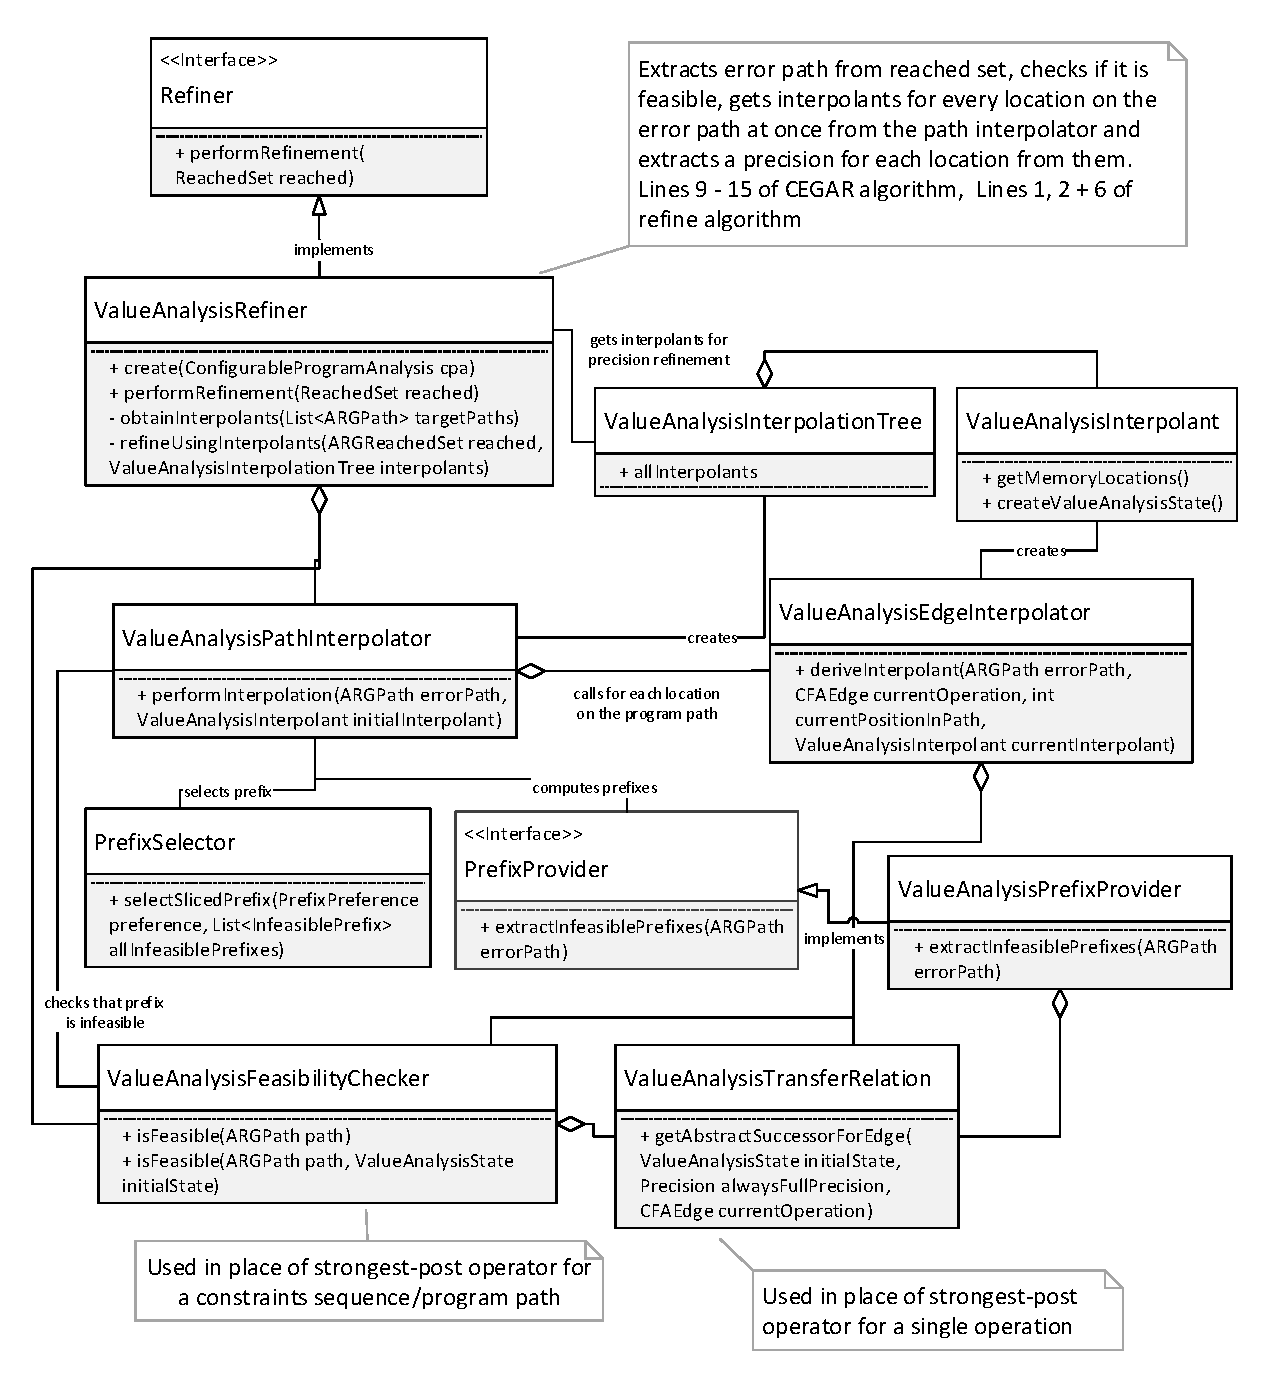
\includegraphics[width=\linewidth]{implementationCegar/ValueAnalysisRefinementBefore}
\caption{Structure of \valueAnalysisCPA\ refinement before refactoring}
\label{fig:valRefinementBefore}
\end{figure}

Keeping these points  in mind, we first take a look at the old structure of the \valueAnalysisCPA's refinement implementation.

\subsection{Structure of \valueAnalysisCPA\ refinement}
Figure \ref{fig:valRefinementBefore} shows the structure of the default refinement procedure for the \valueAnalysisCPA.
The class \objectName{ValueAnalysisRefiner}\ is acting as interface for the refinement procedure.
A deviation from the CEGAR algorithm (Alg.~\ref{alg:cegar}) is that the refinement procedure does not get the error path extracted from the reached set, but the reached set itself.
The refinement procedure is responsible for extracting the error path, checking whether it is feasible, updating the precision if it is not and resetting the reached set and waitlist. (Lines~\ref{alg:cegar:extraction}~--~\ref{alg:cegar:end} in Alg.~\ref{alg:cegar}).

Independent of the way the reached set and waitlist are reset, the precision is updated by getting the existing precisions of all locations removed from the reached set and joining them with the newly extracted precision.

A deviation from the \refineExplicitFunc\ algorithm (Alg.~\ref{alg:refinementExplicit}) is that the interpolants for all program locations on the error path are created by the \objectName{Value\-Analysis\-Path\-Inter\-polator} in one go, stored as a \objectName{Value\-Analysis\-Inter\-po\-la\-tion\-Tree}.
It basically represents Lines~\ref{alg:refinementExplicit:loopStart}~--~\ref{alg:refinementExplicit:interpolation} of the refine algorithm, while \objectName{Value\-Analysis\-Edge\-Inter\-polator} is used for concrete interpolation.
The interpolation algorithm (Alg.~\ref{alg:interpolateExplicit}) gets a prefix and a suffix as parameters, with the prefix being combined from the interpolant computed for the last location and the current location's operation. It then applies the strongest-post operator to the complete prefix with an initial abstract variable assignment to get the abstract variable assignment for the current location.
In the implementation, \objectName{Value\-Analysis\-Edge\-Inter\-polator} receives the interpolant and the current operation in form of a CFA edge, separately.
It is possible to recreate a \objectName{Value\-Analysis\-State} from the interpolant class \objectName{Value\-Analysis\-Interpolant}, so the strongest-post operator only has to be applied to the current operation with the reconstructed state as initial one. This way, no redundant computations happen.

\objectName{Value\-Analysis\-Edge\-Inter\-polator} uses the \objectName{Value\-Analysis\-Trans\-fer\-Re\-la\-tion}\ with full precision as strongest-post operator $\strongestPostOpExplicit$ for single operations, as it represents the same semantics. The \objectName{Value\-Analysis\-State} also used in the abstract domain of the \valueAnalysisCPA\ is used to represent abstract variable assignments. A program variable is represented as a \objectName{Me\-mo\-ry\-Lo\-ca\-tion}.
The class \objectName{Value\-Analysis\-Feasibility\-Checker} is used for the feasibility check $\isFeasibleFunc$ (Alg.~\ref{alg:cegar}, Line~\ref{alg:cegar:feasibilityCheck}).
Since it applies the \objectName{Value\-Analysis\-Transfer\-Relation} also representing $\strongestPostOpExplicit$ sequentially to a program path to check whether it is feasible, it is also used as the sequential application of the strongest-post operator on a program path by the  \objectName{Value\-Analysis\-Edge\-Inter\-polator}.
It is not necessary to transform program paths to constraints sequences, as the transfer relation can work on their edges directly.

The interface \objectName{Pre\-fix\-Pro\-vider}, its implementation \objectName{Value\-Analysis\-Pre\-fix\-Pro\-vider} and the class \objectName{Prefix\-Se\-lector}
are used for the selection of an infeasible path prefix of the error path.
Interpolation is then applied to this prefix only instead of the whole path, to have better control of the interpolants produced and the interpolation process itself.
This concept was introduced in \cite{Beyer2015} and will be used by us without modification.
The algorithm for determining infeasible prefixes also uses the strongest-post operator. In the implementation,
\objectName{Value\-Analysis\-Prefix\-Provider} uses the \objectName{Value\-Analysis\-Transfer\-Relation} for this, as all others do.
In addition, the infeasibility of a chosen prefix is checked again by using the \objectName{Value\-Analysis\-Feasibility\-Checker} since it is possible to be feasible due to imprecision when structs or arrays occur.

\begin{figure}
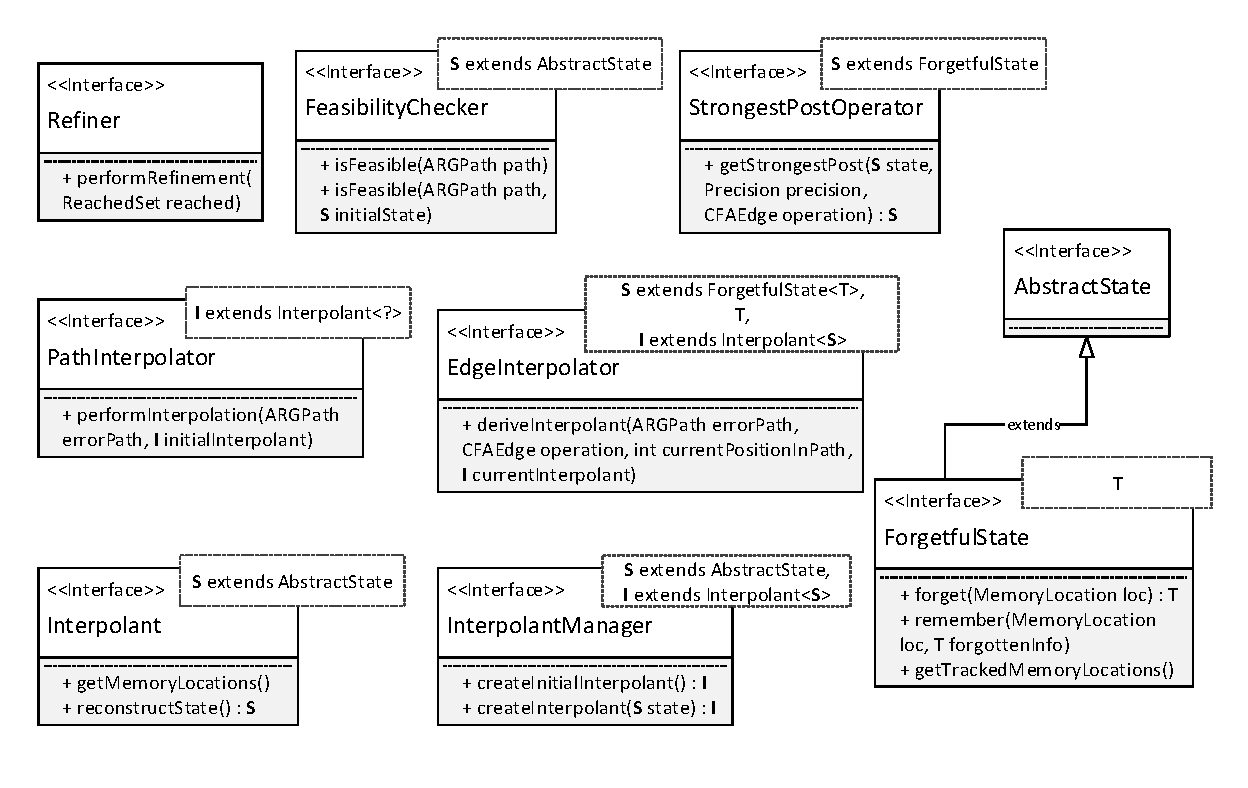
\includegraphics[width=\linewidth]{implementationCegar/RefinementInterfaces}
\caption{Interfaces used in refinement}
\label{fig:refInterfaces}
\end{figure}

\subsection{Introduction of interfaces}
Except for the two classes \objectName{Value\-Analysis\-Refiner} and \objectName{Value\-Analysis\-Prefix\-Provider}, none of these classes are accessed through an interface.
So first, we created interfaces with type parameters that represent all components required for refinement in the domain of abstract variable assignments, based on the existing implementation of the value analysis refinement. These interfaces are displayed in Figure \ref{fig:refInterfaces} next to the \objectName{Refiner} interface.
\objectName{Feasibility\-Checker}, \objectName{Path\-Inter\-po\-lator}, \objectName{Edge\-Inter\-po\-lator}, \objectName{Inter\-po\-lant} are based on their counterpart in value analysis refinement.
The interface \objectName{Strongest\-Post\-Operator} provides the functionality of the strongest-post operator in the refinement algorithms. Its previous counterpart in value analysis refinement is the \objectName{ValueAnalysisTransferRelation} that was used without an interface.
\objectName{Inter\-po\-lant\-Ma\-na\-ger} is an interface providing a previously not needed functionality:
To be able to use an interface for interpolants, this interface is introduced to assume creating them at one point only, through injecting an interpolant manager in other classes of refinement.
\objectName{ForgetfulState} is the interface for states used and created by the \objectName{StrongestPostOperator} and used by the \objectName{EdgeInterpolator}.
It provides means for checking whether an element of the state is needed during interpolation and re-adding it, if it is.

Its type parameter \typeParam{T} describes the type forgotten information is stored in.
The method \objectName{For\-get\-ful\-State.forget(Me\-mo\-ry\-Lo\-ca\-tion)} returns the forgotten information as this type and the type is used to remember the forgotten information, if necessary.
Another type parameter we use is \typeParam{S}, which represents the \objectName{ForgetfulState} implementation used. \objectName{Inter\-po\-lant} and \objectName{Feasibility\-Checker} don't need the additional functionality this interface provides,
so we just use its super-type \objectName{AbstractState} for these.
The third and last type parameter, \typeParam{I}, describes the concrete \objectName{Interpolant} implementation used.
The use of a type parameter describing a concrete implementation instead of just using \objectName{Interpolant<S>} everywhere
allows implementing classes to use methods specific to certain implementations.

\subsection{Creation of generic refinement classes based on refactoring of value analysis refinement}
\begin{figure}[h!]
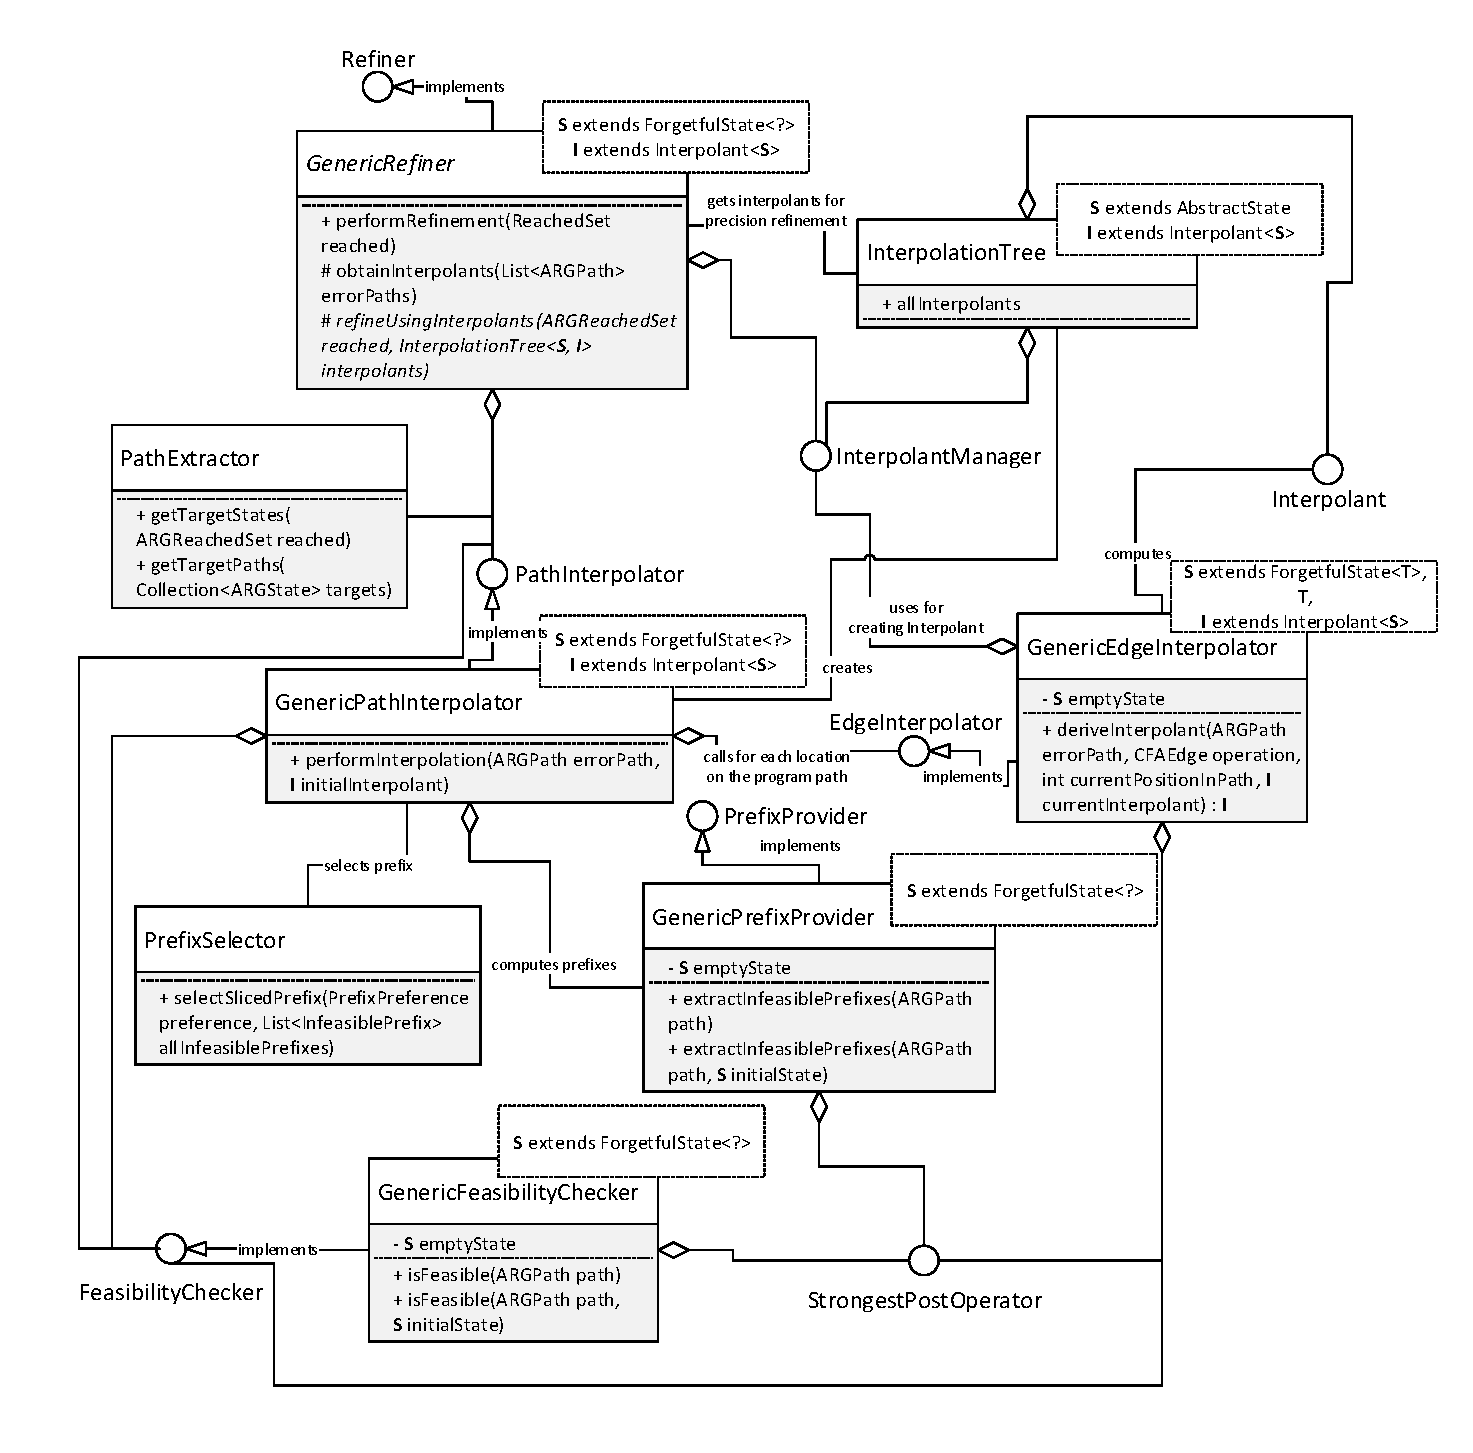
\includegraphics[width=\linewidth]{implementationCegar/RefinementRefactored}
\caption{Structure of generic refinement procedure for abstract variable assignments}
\label{fig:refGeneric}
\end{figure}
After introducing above interfaces, we create new generic refinement classes implementing these interfaces for the domain of abstract variable assignments by using and refactoring most of the code of the existing value analysis refinement.
The resulting structure can be seen in the UML diagram of Figure \ref{fig:refGeneric}.
All aggregation relationships represent dependency injection through the constructor of the classes.
All parts of the refinement procedure are easily interchangeable.
\objectName{GenericRefiner} is an abstract class.
By implementing the method \objectName{refineUsingInterpolants(ARGReachedSet, InterpolationTree)} that is expected to use an interpolation tree to update the precision and reset the reached and waitlist sets represented by the type \objectName{ARGReachedSet}, subtypes can represent a complete refinement procedure.
It is possible to reuse all of the shown classes.
One only has to implement an \objectName{In\-ter\-po\-lant}, a \objectName{For\-get\-ful\-State}, an \objectName{Inter\-po\-lant\-Manager} managing this interpolant type and supporting the state type, and a \objectName{Strong\-est\-Post\-Op\-erator} using the state type.
These types then have to be injected either through the constructor of the \objectName{Generic*} classes, or by choosing the correct type parameter.
